\section{Data Polygon}
\subsection{Data Geospasial}
Istilah ini digunakan karena GIS dibangun berdasarkan pada ‘geografi’ atau ‘spasial’. Object ini mengarah pada spesifikasi lokasi dalam suatu space. Objek bisa berupa fisik, budaya atau ekonomi alamiah. Penampakan tersebut ditampilkan pada suatu peta untuk memberikan gambaran yang representatif dari spasial suatu objek.
Terdapat dua model data geospasial, yaitu model data raster dan model data vektor. 
Pada gambar \ref{datageospasial} dijelaskan tentang Klasifikasi model data geospasial.
\begin{figure}[ht]
	\centerline{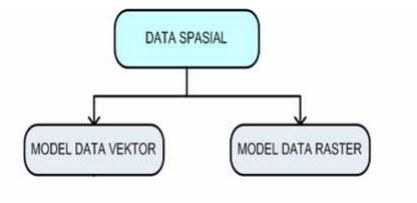
\includegraphics[width=1\textwidth]{figures/datageospasial.JPG}}
	\caption{Klasifikasi Model Data Geospasial.}
	\label{datageospasial}
	\end{figure}

\subsubsection{Data Vektor}
Model data vektor merupakan model data yang paling banyak digunakan dan dikenal pula sebagai model data spaghetti. Lembaran kertas peta ditranslasikan garis demi garis ke dalam list koordinat (x,y) dalam format digital. Sebuah titik dikodekan sebagai pasangan koordinat (x,y) tunggal. Sebuah garis dikodekan sebagai list atau string pasangan koordinat (x,y). Sementara area atau luasan dikodekan sebagai polygon. Data vektor juga merupakan data yang direkam dalam bentuk koordinat titik yang menampilkan, menempatkan dan menyimpan data spesial dengan menggunakan titik, garis atau area (poligon). Ada tiga tipe data vektor (titik, garis, dan poligon) yang bisa digunakan untuk menampilkan informasi pada peta. Titik bisa digunakan sebagai lokasi sebuah kota atau posisi tower radio. Garis bisa digunakan untuk menunjukan route suatu perjalanan atau menggambarkan boundary. Poligon bisa digunakan untuk menggambarkan sebuah danau atau sebuah negara pada peta dunia. Dalam format vektor, bumi direpresentasikan sebagai suatu mosaik dari garis (arc/line), poligon (daerah yang dibatasi oleh garis yang berawal dan berakhir pada titik yang sama), titik/ point (node yang mempunyai lebel), nodes (merupakan titik perpotongan antara dua baris). Setiap bagian dari data vektor dapat saja mempunyai informasi – indormasi yang berasosiasi satu dengan lainnya seperti penggunaan sebuah label untuk menggambarkan informasi pada suatu lokasi. Peta vektor terdiri dari titik, garis, dan area poligon. Bentuknya dapat berupa peta lokal jalan. Kelebihan data vektor yaitu struktur datanya lebih rumit, efisiensi untuk analisis, sebagai sarana representasi yang baik, transformasi proyeksi lebih efisien, ketelitian, akurat dan lebih presisi serta relasi atribut langsung dengan DBMS (database). Adapun kekurangan data vektor adalah sulit dalam melakukan proses overlay, idak bisa menampilkan data image/foto udara, struktur data yang terlalu banyak tidak efektif dalam menampilkan banyak spasial, memerlukan algoritma dan proses yang sangat kompleks, kualitas (output) sangat bergantung dengan printer dan kartografi dan sulit dilakukan simulasi.
Model ini berbasiskan pada titik dengan nilai koordinat (x,y) untuk membangun objek spasialnya. Objek yang dibangun terbagi menjadi tiga bagian lagi yaitu berupa titik (point), garis (line), dan area (polygon).


\subsubsubsection{Polygon}
Dalam artikel Mahendra menjelaskan Polygon merupakan representasi objek dalam dua dimensi. Contoh : danau,
persil tanah, dan lain-lain. Entity polygon dapat direpresentasikan dengan berbagai cara di dalam model data vektor. 
Polygon berasal dari kata Poly yaitu banyak dan gon(gone) yaitu titik. Yang dimaksud adalah polygon yang digunakan sebagai kerangka dasar pemetaan yang memliki titik-titik dimana titik tersebut mempunyai sebuah koordinat X dan Y. 

\subsubsubsection{Jenis - jenis Polygon}
\begin{enumerate}
\item Polygon tertutup
  Polygon Tertutup adalah suatu polygon dimana titik awal dan titik akhir mempunyai posisi yang sama atau berhimpit, sehingga polygon ini adalah suatu rangkain tertutup.
\item Polygon tertutup(koordinat lokal)
  Poligon tertutup yang terikat oleh azimuth dan koordinat.
\item Polygon terbuka tidak terikat/lepas(koordinat lokal)
  Poligon terbuka tanpa ikatan sama sekali (poligon lepas), pengukuran seperti ini akan terjadi pada daerah-daerah yang tidak ada titik tetapnya dan sulit melakukan pengukuran baik dengan cara astronomis maupun dengan satelit. Poligon semacam ini dihitung dengan orientasi lokal artinya koordinat dan azimuth awalnya dimisalkan sembarang.
\item Polygon terbuka tidak terikat sempurna
  Poligon terbuka yang salah satu ujungnya terikat oleh azimuth saja, sedangkan ujung yang lain tidak terikat sama sekali. Poligon semacam ini dapat dihitung dari azimuth awal dan yang diketahui dan sudut-sudut poligon yang diukur, sedangkan koordinat dari masingmasing titiknya masih lokal. Poligon terbuka yang salah satu ujungnya terikat oleh koordinat saja, sedangkan ujung yang lain tidak terikat sama sekali.Poligon semacam ini dapat dihitung dengan cara memisalkan azimuth awal sehingga masing-masing azimuth sisi poligon dapat dihitung, sedangkan koordinat masing-masing titik dihitung berdasarkan koordinat yang diketahui. Oleh karena itu pada poligon bentuk ini koordinat yang dianggap betul hanyalah pada koordinat titik yang diketahui (awal) sehingga poligon ini tidak ada orientasinya.
\item Polygon terbuka terikat sempurna.
  Suatu poligon yang terikat sempurna dapat terjadi pada poligon tertutup ataupun poligon terbuka, suatu titik dikatakan sempurna sebagai titik ikat apabila diketahui koordinat dan jurusannya minimum 2 buah titik ikat dan tingkatnya berada diatas titik yang akan dihasilkan.Poligon terbuka yang masing-masing ujungnya terikat azimuth dan koordinat.
\end{enumerate}

Serangkaian titik-titik yang dihubungkan dengan garis lurus sehingga titik-titik tersebut membentuk sebuh rngkaian(jaringan) ttitkk atau polygon. Pada pekerjaan pembuatan peta, rangkaian titik polygon digunakan sebagai  kerangka peta, yaitu merupakan jaringan titik-titik yang telah tertentu letaknya di tanah yang sudah ditandai dengan patok, dimana semua benda buatan manusia seperti jembatan, jalan raya, gedung maupun benda-benda alam seperti danau, bukit, dan sungai akan berorientasikan. Kedudukan benda pada pekerjaan pemetaan biasanya dinyatakan dengan sistem koordinat  kartesius tegak lurus (X,Y) dibidang datar(peta), dengan sumbu X menyataakan arah timur-barat dan sumbu Y menyatakan arah utara - selatan. Koordinat titik-titik polygon harus cukup teliti mengingat ketelitian letak dan ukuran benda - benda yang akan dipetakan sangat tergantung pada ketelitian dan kerangka peta.

\subsubsubsection{Bentuk-bentuk Polygon}
Menurut bentuknya, polygon dibedakan menjadi dua bentuk :
\begin{enumerate}
\item Polygon Terbuka
Polygon terbuka adalah suatu polygon dimana titik awal dan titik akhirnya berbeda. Polygon yang titik awal dan titik akhirnya merupakan titik yang berlainan (bukan satu titik yang sama). Polygon terbuka ini dapat dibagi lebih lanjut berdasarkan peningkatan pada titik - titik(kedua titik ujungnya). Ada peningkatan untuk polygon terbuka yaitu peningkatan koordinat. Peningkatan koordinat pada polygon terbagi menjadi beberapa yaitu, tanpa ikatan sama sekali dan pada salah satu ujung yang lain tanpa ikatan sama sekali. Jenis - jenis polygon terbuka adalah :
- Polygon terbuka terkait sempurna
- Polygon terbuka terikat sepihak
- Polygon terbuka tidak terikat.

\item Polygon Tertutup
Polygon Tertutup adalah suatu polygon dimana titik awal dan titik akhir mempunyai posisi yang sama atau berhimpit, sehingga polygon ini adalah suatu rangkain tertutup. Pada polygon tertutup garis - garis kembali ke titik awal, jadi membentuk segi banyak. Berakhir di stasiun lain yang mempunyai ketelitian letak sama atau lebih besar darpada ketelitian letak titik awal.
Berdasarkan fungsinya, polygon dibedakan menjadi :
- Polygon untuk keperluan keranga peta, syaratnya harus memiliki titik - titik yang cukup baik, dalam arti menjangkau semua wilayah.
- Polygon yang berfungsi sebagai titik - titik pertolongan untuk mengambil detail lapangan.
Kelememahan polygon tertutup yaitu, bila ada kesalahan yang profesional dengan jarak (salah  satu sistematis) tidak akan ketahuan. Dengan kata lain, walaupun ada esalahan, namun polygon tertutup kelihatan baik juga. Jarak - jarak yang diukur secara elektronis sangat mudah dhinggapi kesalahan seperti kesalahan frekuensi gelombang.
\end{enumerate}

\subsubsubsection{Karakteristik Polygon}
\begin{enumerate}
\item Titik distrukturisasi dan disimpan (direcord) sebagai satu pasang koordinat(x,y).
\item Garis distrukturisasi dan disimpan sebagai suatu susunan pasangan koordinat(x,y) yang beraturan.
\item Luasan distrukturisasi dan disimpan sebagai satuan susunan pasangan koordinat(x,y) yang berurutan yang menyatakan segmen-segmen garis yang menutup menjadi suatu poligon.
\item Data dalam bentuk poligon (area), meliputi daerah administrasi, geologi, geomorfologi, jenis tanah, dan penggunaan tanah. 
\item Data dalam bentuk pixel (grid) meliputi citra satelit dan foto udara. Data dasar yang dimasukan dalam SIG diperoleh dari tiga sumber, yaitu data lapangan (terestris), data peta, dan data penginderaan jauh.
\end{enumerate}

Struktur data polygon bertujuan untuk mendeskripsikan properties yang bersifat topologi dari suatu area sedemikian rupa sehingga properties yang dimiliki oleh blok-blok bangunan spasial dasar dapat ditampilkan dan dimanipulasi sebagai data peta tematik. Seperti halnya titik dan garis, area juga dapat menggambarkan objek yang berbeda menurut skalanya. Area dapat menggambarkan wilayah hutan atau sawah pada peta skala besar.  Poligon-poligon didefinisikan dengan menggunakan arcs:-- dengan melakukan tracing batas-batasnya searah dengan perputaran jarum jam (clockwise), merekam komponen arc beserta orientasinya, memberikan tanda negative pada arcs yang mendefinisikan batas-batas internal.  
Dalam GIS istilah poligon adalah kjumpulan pasangan koordinat yang menghubungkan paling sedikit tiga titik (vertex) dan titik awal bertemu dengan titik yang paling akhir dan menutup. Misalnya : Batas Administrasi
Region, merupakan sekumpulan poligon, di mana masing – masing poligon tersebut dapat atau tidak mempunyai keterikatan di antaranya akan tetapi saling bertampalan dalam satu data set.
Cara yang paling sederhana untuk merepresentasikan suatu poligon adalah pengembangan dari cara yang digunakan untuk merepresentasikan arc yang sederhana yaitu merepresentasikan setiap poligon sebagai sekumpulan koordinat (x,y) yang membentuk segmen garis, dimana mempunyai titik awal dan titik akhir segmen garis yang sama (memiliki nilai koordinat yang sama). Bentuk-bentuk dasar representasi data spasial ini, di dalam sistem model data vektor, didefinisikan oleh sistem koordinat kartesian dua dimensi (x,y). Di dalam model data spasial vektor, garis-garis atau kurva merupakan sekumpulan titik-titik terurut yang dihubungkan. Sedangkan luasan atau poligon juga disimpan sebagai sekumpulan list titik-titik, tetapi dengan catatan bahwa titik awal dan titik akhir poligon memiliki nilai koordinat yang sama dengan syarat poligon tersebur tertutup. Representasi vektor suatu objek merupakan suatu usaha di dalam menyajikan objek yang bersangkutan sesempurna mungkin. Untuk itu, ruang atau dimensi koordinat diasumsikan bersifat kontinyu yang memungkinkan semua posisi, panjang dan dimensi didefinisikan dengan presisi.
Fitur poligon adalah area tertutup seperti bendungan, pulau, batas negara dan sebagainya. Seperti fitur polyline, poligon diciptakan dari rangkaian simpul yang terhubung dengan garis kontinyu. Namun karena poligon selalu menggambarkan area tertutup, simpul pertama dan terakhir harus selalu berada di tempat yang sama! Poligon sering memiliki batas geometri bersama yang sama dengan poligon tetangga. Banyak aplikasi GIS memiliki kemampuan untuk memastikan bahwa batas-batas poligon tetangga persis sama. Kita akan membahasnya di topik Topology nanti di tutorial ini. Seperti halnya titik dan polyline, poligon memiliki atribut. Atribut menggambarkan masing-masing poligon. Misalnya bendungan mungkin memiliki atribut untuk kedalaman dan kualitas air. Format : Koordinat dengan titik awal dan akhir sama, mempunyai panjang dan luasan. Contoh : Tanah persil, bangunan. \cite{mahendra2014sistem}.
